\documentclass{article}
\usepackage{tikz}
\usetikzlibrary{positioning, shapes, arrows, fit, calc, decorations.pathreplacing, calligraphy}
\usepackage[margin=1cm]{geometry}
\usepackage{xcolor}

\begin{document}

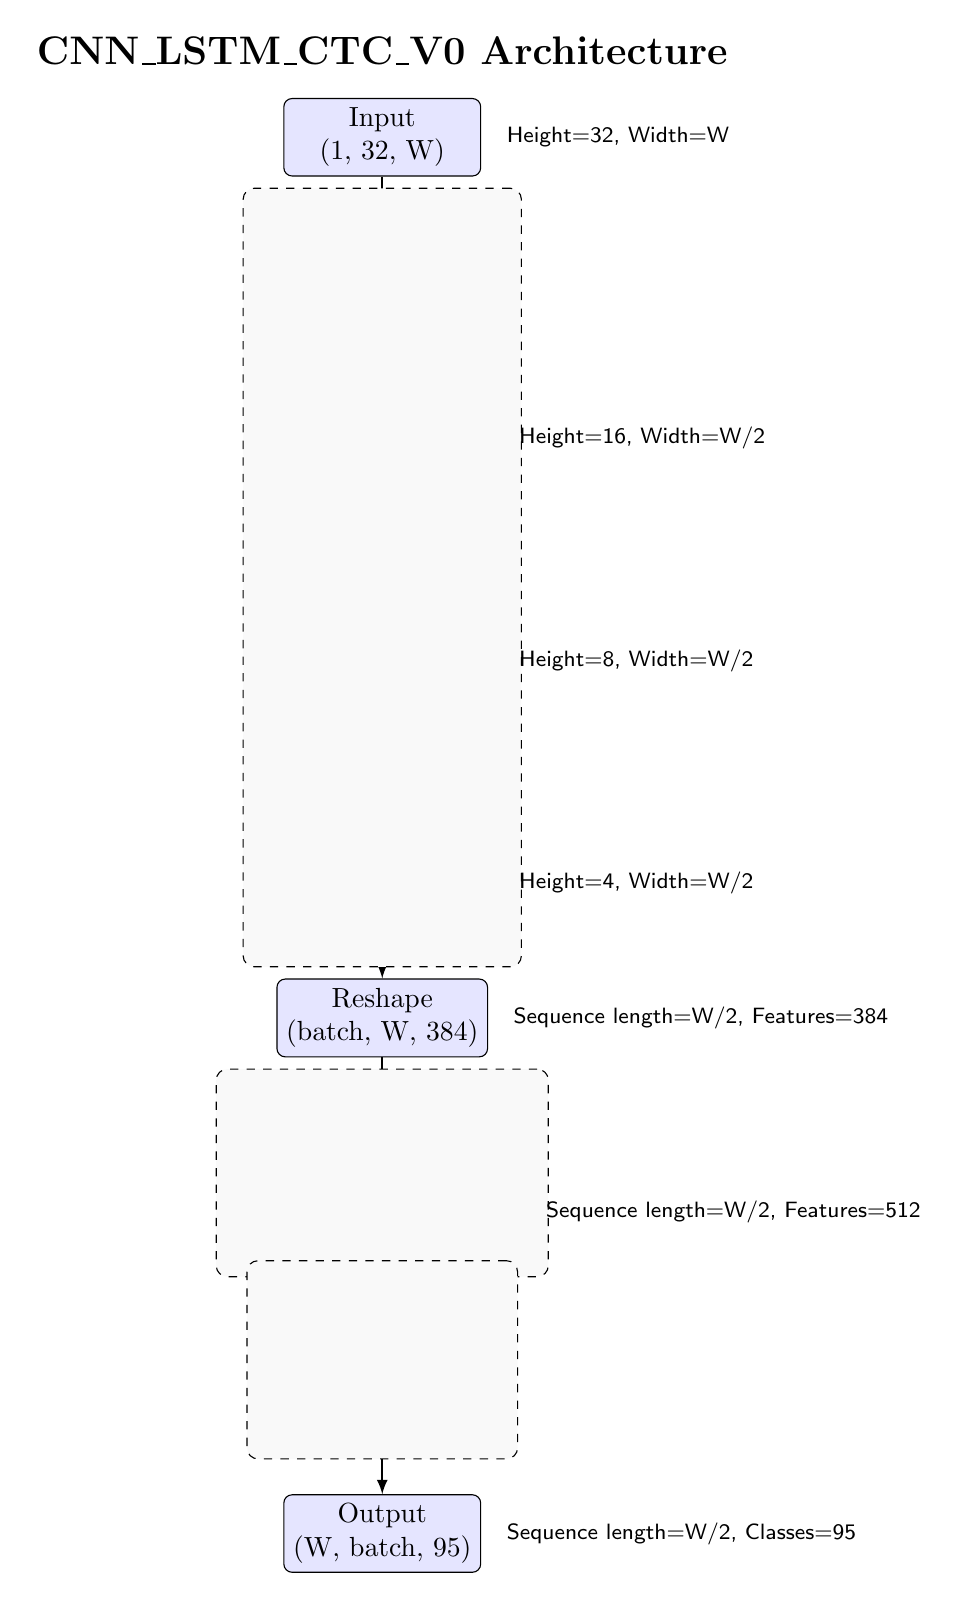
\begin{tikzpicture}[
    node distance=0.8cm,
    box/.style={draw, minimum width=2.5cm, minimum height=0.8cm, align=center, rounded corners=3pt, fill=blue!10},
    conv/.style={box, fill=green!20},
    pool/.style={box, fill=cyan!20},
    lstm/.style={box, fill=orange!20, minimum width=3.5cm},
    fc/.style={box, fill=red!20},
    groupbox/.style={draw, dashed, rounded corners, inner sep=10pt, fill=gray!5},
    arr/.style={->, >=latex, thick},
    label/.style={font=\footnotesize\sffamily}
]

% Input
\node[box] (input) {Input\\(1, 32, W)};

% CNN Block
\node[groupbox, below=1cm of input, label={[anchor=north west]north west:CNN Block (10.6\% params)}] (cnn_block) {};

% First Conv+ReLU+Conv+ReLU+MaxPool block
\node[conv, below=1.5cm of input] (conv1) {Conv2d(1$\rightarrow$24)};
\node[pool, below=0.6cm of conv1] (pool1) {MaxPool2d(2, 2)};

% Second Conv+ReLU+Conv+ReLU+MaxPool block
\node[conv, below=0.6cm of pool1] (conv2) {Conv2d(24$\rightarrow$48)};
\node[pool, below=0.6cm of conv2] (pool2) {MaxPool2d(2, 1)};

% Third Conv+ReLU+Conv+ReLU+MaxPool block
\node[conv, below=0.6cm of pool2] (conv3) {Conv2d(48$\rightarrow$96)};
\node[pool, below=0.6cm of conv3] (pool3) {MaxPool2d(2, 1)};

% Reshape
\node[box, below=0.8cm of pool3] (reshape) {Reshape\\(batch, W, 384)};

% LSTM Block
\node[groupbox, below=1cm of reshape, label={[anchor=north west]north west:LSTM Block (86.2\% params)}] (lstm_block) {};
\node[lstm, below=1.5cm of reshape] (lstm) {LSTM(384$\rightarrow$256)\\Bidirectional};

% FC Block
\node[groupbox, below=1cm of lstm, label={[anchor=north west]north west:FC Block (3.2\% params)}] (fc_block) {};
\node[fc, below=1.5cm of lstm] (fc) {Linear(512$\rightarrow$95)};

% Output
\node[box, below=0.8cm of fc] (output) {Output\\(W, batch, 95)};

% Connections
\draw[arr] (input) -- (conv1);
\draw[arr] (conv1) -- (pool1);
\draw[arr] (pool1) -- (conv2);
\draw[arr] (conv2) -- (pool2);
\draw[arr] (pool2) -- (conv3);
\draw[arr] (conv3) -- (pool3);
\draw[arr] (pool3) -- (reshape);
\draw[arr] (reshape) -- (lstm);
\draw[arr] (lstm) -- (fc);
\draw[arr] (fc) -- (output);

% Adjust group boxes to encompass their contents
\coordinate (cnn_top) at ($(input.south) + (0,-0.5)$);
\coordinate (cnn_bottom) at ($(reshape.north) + (0,0.5)$);
\node[groupbox, fit=(cnn_top) (conv1) (pool1) (conv2) (pool2) (conv3) (pool3) (cnn_bottom), label={[anchor=north west]north west:CNN Block (10.6\% params)}] (cnn_block) {};

\coordinate (lstm_top) at ($(reshape.south) + (0,-0.5)$);
\coordinate (lstm_bottom) at ($(lstm.south) + (0,0.5)$);
\node[groupbox, fit=(lstm_top) (lstm) (lstm_bottom), label={[anchor=north west]north west:LSTM Block (86.2\% params)}] (lstm_block) {};

\coordinate (fc_top) at ($(lstm.south) + (0,-0.5)$);
\coordinate (fc_bottom) at ($(fc.south) + (0,0.5)$);
\node[groupbox, fit=(fc_top) (fc) (fc_bottom), label={[anchor=north west]north west:FC Block (3.2\% params)}] (fc_block) {};

% Title
\node[align=center, font=\Large\bfseries, above=0.3cm of input] {CNN\_LSTM\_CTC\_V0 Architecture};

% Data dimensions annotations
\node[label, right=0.2cm of input] {Height=32, Width=W};
\node[label, right=0.2cm of pool1] {Height=16, Width=W/2};
\node[label, right=0.2cm of pool2] {Height=8, Width=W/2};
\node[label, right=0.2cm of pool3] {Height=4, Width=W/2};
\node[label, right=0.2cm of reshape] {Sequence length=W/2, Features=384};
\node[label, right=0.2cm of lstm] {Sequence length=W/2, Features=512};
\node[label, right=0.2cm of output] {Sequence length=W/2, Classes=95};

\end{tikzpicture}

\end{document}